\documentclass[reqno, 11pt]{amsart}
\usepackage{amssymb}
\usepackage{tikz, pgfplots}
\usetikzlibrary{positioning}
\usetikzlibrary{calc}
\usetikzlibrary{patterns}
\usetikzlibrary{patterns.meta}
\pgfplotsset{compat=1.18}

\newcommand{\Imm}{\operatorname{Im}}

\newcommand{\Ree}{\operatorname{Re}}

\begin{document}

    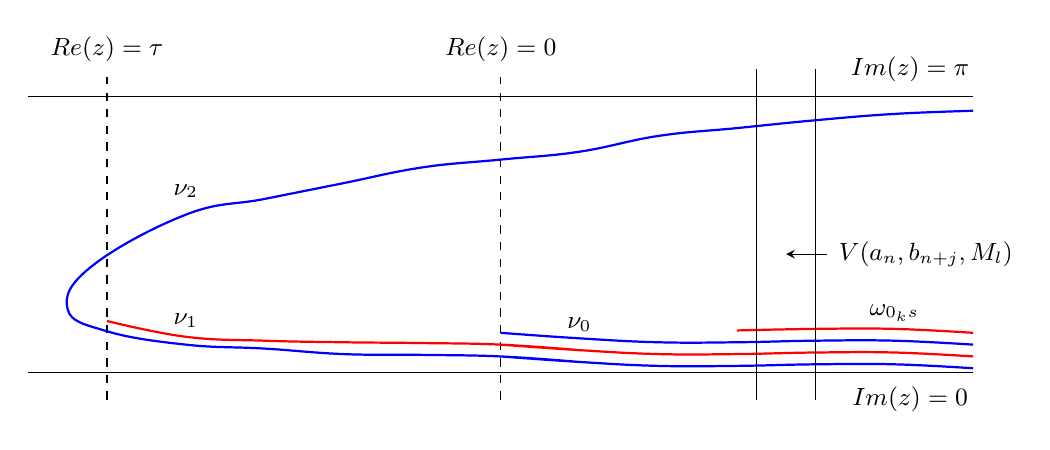
\begin{tikzpicture}[font=\small]

    \draw (-2,2) -- (10,2);
    \draw (-2,-1.5) -- (10,-1.5);

    \draw node at (9.2,2.35) {$\Imm(z)=\pi$};    
    \draw node at (9.2,-1.85){$\Imm(z)=0$};

    \draw [dashed] (4,-1.85) -- (4,2.25);
    \draw [dashed] (-1,-1.85) -- (-1,2.25);

    \draw node at (4,2.6) {$\Ree(z)=0$};
    \draw node at (-1,2.6) {$\Ree(z)=\tau$};

    \draw [thick, blue] plot [smooth, tension=0.7] coordinates {(10,-1.45) (9,-1.4) (8,-1.4) (7,-1.42) (6,-1.42) (5,-1.37) (4,-1.30) (5,-1.37) (4,-1.30) (3,-1.28) (2,-1.27) (1,-1.20) (0,-1.15) (-1,-0.98) (-1.5,-0.7) (-1.2,-0.16) (0,0.5) (1,0.7) (2,0.9) (3, 1.1) (4,1.2) (5,1.3) (6,1.5) (7,1.6) (8,1.7) (9,1.78) (10,1.82)};

    \draw [thick, red] plot [smooth, tension=0.7] coordinates {(10,-1.30) (9,-1.25) (8,-1.25) (7,-1.27) (6,-1.27) (5,-1.22) (4,-1.15) (5,-1.22) (4,-1.15) (3,-1.13) (2,-1.12) (1,-1.10) (0,-1.05) (-1,-0.85)};

    \draw [thick, blue] plot [smooth, tension=0.7] coordinates {(10,-1.15) (9,-1.1) (8,-1.1) (7,-1.12) (6,-1.12) (5,-1.07) (4,-1)};

    \draw [thick, red] plot [smooth, tension=0.7] coordinates {(10,-1) (9,-0.95) (8,-0.95) (7,-0.97)};

    \draw node at (9,-0.75) {$\omega_{0_ks}$};
    \draw node at (5,-0.9) {$\nu_{0}$};
    \draw node at (0,-0.85) {$\nu_{1}$};
    \draw node at (0,0.8) {$\nu_{2}$};

    \draw (7.25,-1.85) -- (7.25,2.35);
    \draw (8,-1.85) -- (8,2.35);

    \draw node at (9.4,0) {\small $V(a_n,b_{n+j},M_l)$};
    \draw [-stealth](8.15,0) -- (7.625,0);

\end{tikzpicture}

\end{document}